\documentclass{standalone}

\usepackage{tikz}
\usepackage{pgfplots}
\usepackage{xcolor}

\begin{document}

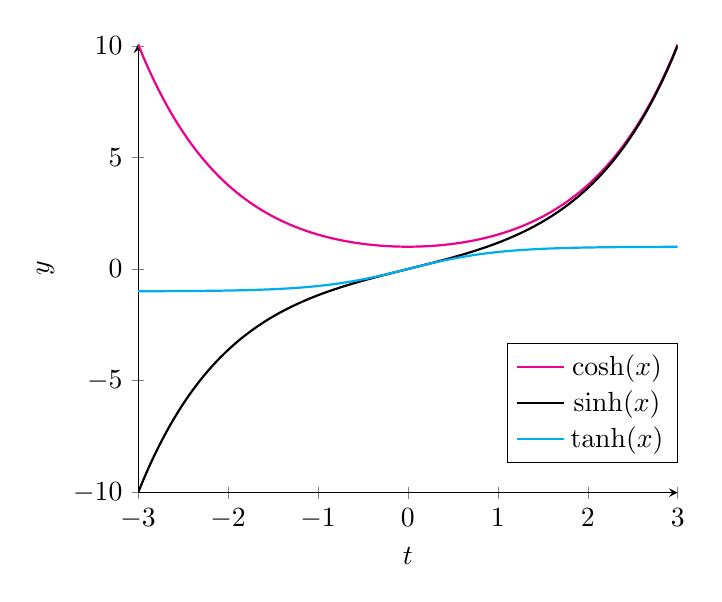
\begin{tikzpicture}
  \begin{axis}[
    domain=-3:3,
    samples=100,
    axis lines=left,
    xlabel=$t$,
    ylabel=$y$,
    legend style={at={(1,0.2)}, anchor=east},
  ]
  
  % Define a list of colors
  
  \addplot[magenta, thick] {cosh(x)}; 
  \addlegendentry{$\cosh(x)$}
  
  \addplot[black, thick] {sinh(x)}; 
  \addlegendentry{$\sinh(x)$}
  
  \addplot[cyan, thick] {tanh(x)}; 
  \addlegendentry{$\tanh(x)$}
  
  \end{axis}
\end{tikzpicture}

\end{document}
